% generated by paper/derive.py from results/p2-games.jsonl; do not edit
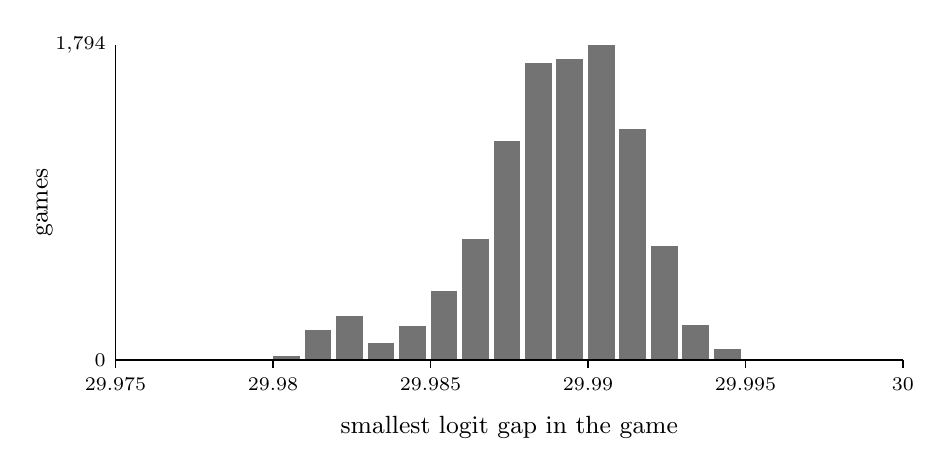
\begin{tikzpicture}
\fill[black!55] (0.000,0) rectangle +(0.340,0.000);
\fill[black!55] (0.400,0) rectangle +(0.340,0.000);
\fill[black!55] (0.800,0) rectangle +(0.340,0.000);
\fill[black!55] (1.200,0) rectangle +(0.340,0.000);
\fill[black!55] (1.600,0) rectangle +(0.340,0.011);
\fill[black!55] (2.000,0) rectangle +(0.340,0.054);
\fill[black!55] (2.400,0) rectangle +(0.340,0.379);
\fill[black!55] (2.800,0) rectangle +(0.340,0.562);
\fill[black!55] (3.200,0) rectangle +(0.340,0.212);
\fill[black!55] (3.600,0) rectangle +(0.340,0.433);
\fill[black!55] (4.000,0) rectangle +(0.340,0.872);
\fill[black!55] (4.400,0) rectangle +(0.340,1.536);
\fill[black!55] (4.800,0) rectangle +(0.340,2.778);
\fill[black!55] (5.200,0) rectangle +(0.340,3.773);
\fill[black!55] (5.600,0) rectangle +(0.340,3.822);
\fill[black!55] (6.000,0) rectangle +(0.340,4.000);
\fill[black!55] (6.400,0) rectangle +(0.340,2.939);
\fill[black!55] (6.800,0) rectangle +(0.340,1.449);
\fill[black!55] (7.200,0) rectangle +(0.340,0.450);
\fill[black!55] (7.600,0) rectangle +(0.340,0.134);
\fill[black!55] (8.000,0) rectangle +(0.340,0.009);
\fill[black!55] (8.400,0) rectangle +(0.340,0.000);
\fill[black!55] (8.800,0) rectangle +(0.340,0.000);
\fill[black!55] (9.200,0) rectangle +(0.340,0.000);
\fill[black!55] (9.600,0) rectangle +(0.340,0.000);
\draw (0,0) -- (10.0,0);
\draw (0.000,0) -- +(0,-0.1) node[below] {\scriptsize 29.975};
\draw (2.000,0) -- +(0,-0.1) node[below] {\scriptsize 29.98};
\draw (4.000,0) -- +(0,-0.1) node[below] {\scriptsize 29.985};
\draw (6.000,0) -- +(0,-0.1) node[below] {\scriptsize 29.99};
\draw (8.000,0) -- +(0,-0.1) node[below] {\scriptsize 29.995};
\draw (10.000,0) -- +(0,-0.1) node[below] {\scriptsize 30};
\node at (5.0,-0.85) {\small smallest logit gap in the game};
\draw (0,0) -- (0,4.0);
\node[left] at (0,4.0) {\scriptsize 1,794};
\node[left] at (0,0) {\scriptsize 0};
\node[rotate=90] at (-0.9,2.0) {\small games};
\end{tikzpicture}
